\documentclass[aspectratio=169, fleqn, 10pt]{beamer}
\usepackage[utf8]{inputenc}
\usepackage[english]{babel}
\usepackage{amsmath}
\usepackage{amsfonts}
\usepackage{amssymb}
\usepackage{bm}
\usepackage{graphicx}

\usepackage{caption} % add the caption* command
\usepackage{hyperref}
\usepackage{tikz}
\usepackage{verbatim}
\usetikzlibrary{arrows,shapes}

% beamer conf
\usetheme{Warsaw}%{Pittsburgh}%%{CambridgeUS}%{default}%
\usecolortheme{seahorse}
\usefonttheme{professionalfonts}

%tikz configuration
\usetikzlibrary{arrows,matrix,positioning,fit}
\tikzset{highlight/.style={rectangle,rounded corners,fill=red!15,draw,fill opacity=0.5,thick,inner sep=0pt}}
\newcommand{\tikzmark}[2]{\tikz[overlay,remember picture,baseline=(#1.base)] \node (#1) {#2};}
%
\newcommand{\Highlight}[1][submatrix]{%
    \tikz[overlay,remember picture]{
        \node[highlight,fit=(left.north west) (right.south east)] (#1) {};}
}

% code from http://tex.stackexchange.com/questions/110720/adding-a-take-away-box-to-a-beamer-slide
\makeatletter
\newcommand\insertimptext[1]{
	\begin{tikzpicture}[remember picture,overlay]
	\node[inner sep=0pt,outer sep=0pt,anchor=south] at ([yshift=20pt]current page.south)
	{\begin{beamercolorbox}[wd=0.65\paperwidth,ht=3ex,dp=2ex,center]{author in head/foot}
		\hfill\parbox[c][7ex][c]{0.6\paperwidth}{\centering\footnotesize#1}\hfill\null
		\end{beamercolorbox}
	};
	\end{tikzpicture}%
}
\makeatother
%setbeamercovered{transparent}
%setbeamertemplate{navigation symbols}{}

\newcommand{\mat}[1]{\begin{bmatrix}#1\end{bmatrix}}

\title{Heuristic on state estimation}
\author{Luca Parolini}
\date{\today}

\begin{document}
	
% code taken from http://www.texample.net/tikz/examples/beamer-arrows/
% For every picture that defines or uses external nodes, you'll have to
% apply the 'remember picture' style. To avoid some typing, we'll apply
% the style to all pictures.
\tikzstyle{every picture}+=[remember picture]
\tikzstyle{myarrows}=[line width=1mm,draw=blue!20,fill opacity=0.8,-triangle 45,postaction={draw, line width=3mm, shorten >=4mm, -}]
\tikzstyle{na} = [baseline=-.5ex]
\tikzstyle{block} = [draw, fill=blue!20, rectangle, minimum width=2em] %, 
\tikzstyle{sum} = [draw, fill=blue!20, circle] %, node distance=1cm
\tikzstyle{input} = [coordinate]
\tikzstyle{output} = [coordinate]
\tikzstyle{pinstyle} = [pin edge={to-,thin,black}]

% By default all math in TikZ nodes are set in inline mode. Change this to
% displaystyle so that we don't get small fractions.
%\everymath{\displaystyle}

\maketitle
%\frame{\tableofcontents[currentsection]}
\section{Deterministic approach}
\begin{frame} 
	\frametitle{Speed estimation from position measurements} 
	Consider a car and a (quite inaccurate) model of it
	\begin{columns}[onlytextwidth]
		\column{.4\textwidth}
		\begin{figure}[h]
			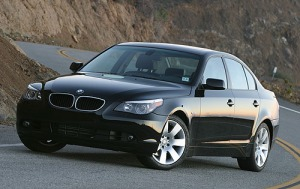
\includegraphics[width=\textwidth]{fig/auto_real}%
			\caption*{The car we want to model.\footnotemark} 
		\end{figure}
		\column{.1\textwidth}
		\begin{tikzpicture}
		\draw [myarrows] (0, 0) -- (1, 0);
		\end{tikzpicture}
		\column{.4\textwidth}
		\begin{block}{The (quite inaccurate) model}
		Position at time $t$: $(\xi(t), \zeta(t))$ \\%{\footnotesize ($x$ and $y$  will be used later with different a meaning)}\\
		Equations of motion:
		\begin{align*}
		  \ddot{\xi}(t)& = u_1(t) \\
		  \ddot{\zeta}(t)& = u_2(t)
		\end{align*}
		where 
		\begin{itemize}
			%\item $M$ mass of the car\\
			\item $u_1(t)$ acceleration along first coordinate, i.e. $\xi$\\
			\item $u_2(t)$ acceleration along scond coordinate, i.e. $\zeta$ 
		\end{itemize}
		These are the control inputs.
		\end{block}
	\end{columns}
	
	
	\footnotetext{\href{https://commons.wikimedia.org/wiki/File\%3A2015_BMW_i8_(20039281571)_(2).jpg}{\tiny{Image by Edvvc from London, UK (2015 BMW i8)}}}
\end{frame}

\begin{frame} 
	\frametitle{Model rewriting in state space form}
	It will be convenient in the following, to rewrite the model in a more standard form
    \begin{columns}[onlytextwidth]
    \column{.25\textwidth}
        \begin{align*}
        \ddot{\xi}(t)& = \frac{1}{M} u_1(t) \\
        \ddot{\zeta}(t)& = \frac{1}{M} u_2(t)
        \end{align*}
    \column{.1\textwidth}
    \begin{tikzpicture}
        \draw [myarrows] (0, 0) -- (1, 0);
    \end{tikzpicture}
    \column{.8\textwidth}
    	\begin{align*}
    	  \mat{\dot{\xi}\\\ddot{\xi}\\\dot{\zeta}\\\ddot{\zeta}}&=
          \mat{0&1&0&0\\0&0&0&0\\0&0&0&1\\0&0&0&0}\mat{\xi\\\dot{\xi}\\{\zeta}\\\dot{\zeta}} + \mat{0&0\\ \frac{1}{M} &0\\0&0 \\0&\frac{1}{M}} \mat{u_1(t)\\u_2(t)}\\
          \mat{y_1(t)\\y_2(t)}&=\mat{1&0&0&0\\0&0&1&0}\mat{\xi\\\dot{\xi}\\{\zeta}\\\dot{\zeta}}
    	\end{align*}
    \end{columns}
\end{frame}

\begin{frame} 
    \frametitle{Model rewriting}
    It will be convenient in the following, to rewrite the model in a more standard form
    \begin{columns}[onlytextwidth]
        \column{.2\textwidth}
        \begin{align*}
        \ddot{\xi}(t)& = \frac{1}{M} u_1(t) \\
        \ddot{\zeta}(t)& = \frac{1}{M} u_2(t)
        \end{align*}
        \vspace*{2em}
        \column{.1\textwidth}
        \begin{center}
           \begin{tikzpicture}
           \draw [myarrows] (0, 0) -- (1, 0);
           \end{tikzpicture} 
        \end{center}
        \vspace*{1em}
        \column{.6\textwidth}
        \begin{align*}
        \mat{\dot{\xi}\\\ddot{\xi}\\\dot{\zeta}\\\ddot{\zeta}} 
        &=
        \mat{0&1&0&0\\0&0&0&0\\0&0&0&1\\0&0&0&0}
        \tikz[baseline]{
            \node[fill=blue!10,anchor=base,rounded corners] (state)
            {$\mat{{\xi}\\\dot{\xi}\\{\zeta}\\\dot{\zeta}}$};
        }
        + 
        \mat{0&0\\ \frac{1}{M} &0\\0&0 \\0&\frac{1}{M}} 
        \tikz[baseline]{
            \node[fill=blue!10,anchor=base,rounded corners] (input)
            {$\mat{u_1(t)\\u_2(t)}$};
        }\\
        \tikz[baseline]{
            \node[fill=blue!10,anchor=base,rounded corners] (output)
            {$\mat{y_1(t)\\y_2(t)}$};
        }
        &=\mat{1&0&0&0\\0&0&1&0}\mat{\xi\\\dot{\xi}\\{\zeta}\\\dot{\zeta}}
        \end{align*}
        
        
        \begin{minipage}{5cm}\hfill\end{minipage}
        \begin{minipage}{3cm}
        \tikz[na]\node (statedef) {$\bm{x}(t)$: state};\vspace{-0.8em} 
        \tikz[na]\node (inputdef) {$\bm{u}(t)$: input};\vspace{-0.8em}
        \tikz[na]\node (outputdef) {$\bm{y}(t)$: output}; 
        \end{minipage}        
    \end{columns}
    \begin{tikzpicture}[overlay]
        \path[->](state) edge (statedef);
        \path[->](input) edge [out=-90, in=0] (inputdef);
        \path[->](output) edge [out=-90, in=-180] (outputdef);
    \end{tikzpicture}
\end{frame}

\begin{frame} 
    \frametitle{State space form}
    The names $A$, $B$, $C$ are often used in state space form. We can write 
    \begin{align*}
    \dot{\bm{x}}(t) &= A \bm{x}(t) + B \bm{u}(t)\\
    \bm{y}(t) &= C \bm{x} (t)
    \end{align*}
    \begin{columns}    %[onlytextwidth,t]
    \column{.4\textwidth}
        where 
        \begin{itemize}
            \item ${\bm{x}}(t)=\mat{{\xi}\\\dot{\xi}\\{\zeta}\\\dot{\zeta}}$ state of the system
            \item ${\bm{y}}(t)=\mat{y_1(t)\\y_2(t)}$ measured output
            \item ${\bm{u}}(t)=\mat{u_1(t)\\u_2(t)}$ input
        \end{itemize}
    \column{.5\textwidth}
    A graphical representation can be given as
    %\begin{block}
        \begin{tikzpicture}[auto,  >=latex']
        \node [input, name=input] {};
        \node [block, right of=input] (blockB) {$B$};
        \node [sum, right of=blockB] (sum) {};
        \node [input, right of=sum] (dstate) {$\frac{1}{s}$};
        \node [block, right of=dstate] (integrator) {$\frac{1}{s}$};
        \node [input, right of=integrator] (state) {};
        \node [block, right of=state] (blockC) {$C$};
        \node [block, below of=integrator] (blockA) {$A$};
        \node [output, right of=blockC] (output) {};
        
        \draw [draw,->] (input) -- node {$\bm{u}(t)$} (blockB);
        \draw [->] (blockB) -- node {} (sum);
        \draw [->] (sum) -- node {$\dot{\bm{x}}(t)$} (integrator);
        \draw [->] (integrator) -- node {$\bm{x}(t)$} (blockC);
        \draw [->] (blockC) -- node [name=y] {  $\bm{y}(t)$}(output);
        \draw [->] (state) |- node {}(blockA);
        \draw [->] (blockA) -| node[pos=0.99] {$+$} 
        node [near end] {} (sum);
        \end{tikzpicture}
    %\end{block}
    
    Simplified form
    
         \begin{tikzpicture}[auto,  >=latex']
         \node [input, name=input] {};
         \node [block, right of=input] (blockAB) {$A$, $B$};
         \node [input, right of=blockAB] (state) {$x(t)$};
         \node [block, right of=state] (blockC) {$C$};
         \node [output, right of=blockC] (output) {$y(t)$};
         
         \draw [draw,->] (input) -- node {$\bm{u}(t)$} (blockAB);
         \draw [->] (blockAB) -- node {$\bm{x}(t)$} (blockC);
         \draw [->] (blockC) -- node [name=y] {$\bm{y}(t)$}(output);
         \end{tikzpicture}
    \end{columns}
\end{frame}

\begin{frame} 
    \frametitle{Conversion to discrete time}
    Our estimator will be as a discrete time system. We rewrite our original model as a discrete time system. 
    
    \begin{itemize}
        \item $\Delta t$ denotes the length sampling interval
        \item $t_0$ initial time stamp
        \item ${\bm{x}}(k)$ is the $k^{th}$ samples of the state, i.e., $\bm{x}(k)=\bm{x}(t_0+k\Delta t)$. Similar notation for input and output
        \item $A_d$: discrete time version of the matrix $A$
        \item $B_d$: discrete time version of the matrix $B$
    \end{itemize}
     
    \begin{columns}[onlytextwidth]
        \column{.4\textwidth}
        \begin{block}{Continuous time}
            \vspace*{-1em}
            \begin{align*}
            \dot{\bm{x}}(t) &= A \bm{x}(t) + B \bm{u}(t)\\
            \bm{y}(t) &= C \bm{x}(t) 
            \end{align*}
        \end{block}    
        \column{.1\textwidth}
        \begin{tikzpicture}
        \draw [myarrows] (0, 0) -- (1, 0);
        \end{tikzpicture}
        \column{.4\textwidth}
        \begin{block}{Discrete time}
            \vspace*{-1em}
            \begin{align*}
            \bm{x}(k+1) &= A_d \bm{x}(k) + B_d \bm{u}(k)\\
            \bm{y}(k) &= C \bm{x}(k) 
            \end{align*}
        \end{block}
    \end{columns}
\end{frame}

\begin{frame} 
	\frametitle{Conversion to discrete time}
	\begin{columns}[onlytextwidth]
		\column{.4\textwidth}
		\begin{block}{Continuous time}
			\vspace*{-1em}
			\begin{align*}
			\dot{\bm{x}}(t) &= A \bm{x}(t) + B \bm{u}(t)\\
			\bm{y}(t) &= C \bm{x}(t) 
			\end{align*}
			\vspace*{-2em}
			\begin{align*}
			A&=
			\mat{0&1&0&0\\0&0&0&0\\0&0&0&1\\0&0&0&0}
			\\
			B&=\mat{0&0\\ \frac{1}{M} &0\\0&0 \\0&\frac{1}{M}}
			\end{align*}
		\end{block}
		\column{.2\textwidth}
		\centering
		\begin{tikzpicture}
		\draw [myarrows] (0, 0) -- (1, 0);
		\end{tikzpicture}
		\column{.4\textwidth}
		\begin{block}{Discrete time \footnotemark}
			\vspace*{-1em}
			\begin{align*}
			\bm{x}(k+1) &= A_d \bm{x}(k) + B_d \bm{u}(k)\\
			\bm{y}(k) &= C \bm{x}(k) 
			\end{align*}
			\vspace*{-2em}
			\begin{align*}
			A_d&=\mat{1&\Delta t&0&0\\0&1&0&0\\0&0&1&\Delta t\\0&0&0&1}
			\\
			B_d&=\mat{\frac{\Delta t^2}{2}&0\\ \Delta t &0\\0&\frac{\Delta t^2}{2} \\0&\Delta t}
			\end{align*}
		\end{block}
	\end{columns}
\footnotetext{\href{http://users.isy.liu.se/rt/fredrik/edu/sensorfusion/lecture9.pdf}{\small{For the discretization step see e.g., G. Fredrik. \emph{Sensor fusion} (slides)}}}
\end{frame}

\begin{frame}
    \frametitle{Estimation approaches}
    \begin{itemize}
        \item The position of the car is available at every step $k$. Speed could be estimated by numerical differentiation (Numerical differentiation)
        \item We could try to estimate the \emph{whole} state of the system and then, to extract the speed of the car from the estimated state (Observer approach)
    \end{itemize}
     \begin{columns}[t]
        \column{.5\textwidth}
        \begin{block}{1. Numerical differentiation}
            \vspace*{-1em}
            \begin{align*}
            \hat{\dot{\xi}}(k)& = \frac{y_1(k) - y_1(k-1)}{\Delta t}\\
            \hat{\dot{\zeta}}(k)& = \frac{y_2(k) - y_2(k-1)}{\Delta t}
            \end{align*}
        \end{block}
        \column{.5\textwidth}
        \begin{block}{2. Observer}
            First element of the estimated state
            $$\hat{\dot{\xi}}(k)= \hat{x}_1(k)$$
            Third element of the estimated state
            $$\hat{\dot{\zeta}}(k)=\hat{x}_3(k)$$
        \end{block}	
    \end{columns} 
\end{frame}

\begin{frame}
    \frametitle{Observer derivation}
    \begin{columns}
    	\column{.4\textwidth}
			Assume 
			\begin{itemize}
			  \item Model and parameters of the system are known
			  \item Input and output are measured without noise
			  \item An initial estimate of the state is known $\hat{\bm{x}}(0)$ 
			\end{itemize}
			\vspace{1em}
			We could define the observer as\vspace{-0.8em}
			\begin{align*}
				\hat{\bm{x}}(k+1) &= A_d \hat{\bm{x}}(k) + B_d \bm{u}(k)\\
				\hat{\bm{y}}(k) &= C\hat{\bm{x}}(k) 
			\end{align*}
		\column{.4\textwidth}
		\begin{block}{Diagram}
			\hfill \tikz[na]\node (label1) {True model};\vspace{0.8em}	
			\begin{tikzpicture}[auto,  >=latex']
				\node [input, name=input] {};
				\node [input, name=connection, right of=input]{};
				\node [block, right of=connection] (blockAB) {$A_d$, $B_d$};
				\node [input, right of=blockAB] (state) {$x(k)$};
				\node [block, right of=state] (blockC) {$C$};
				\node [output, right = 4em of blockC] (output) {$y(k)$};
				\begin{scope}[on background layer]
				\draw[fill=blue!55, rounded corners] ($(blockAB.north west)+(-0.1,0.4)$)  rectangle ($(blockC.south east)+(0.2,-0.2)$);
				\end{scope}
				
				\draw [draw,->] (input) -- node {$u(k)$} (blockAB);
				\draw [->] (blockAB) -- node {$\bm{x}(k)$} (blockC);
				\draw [->] (blockC) -- node [name=y] {$\bm{y}(k)$}(output);
				
				\node [block, below = 3em of blockAB] (blockObserverAB) {$A_d$, $B_d$};
				\node [block, below = 3em of blockC] (blockObserverC) {$C$};
				\node [output, right = 4em of blockObserverC] (outputObserver) {};
				\begin{scope}[on background layer]
				\draw[fill=red!55, rounded corners] ($(blockObserverAB.north west)+(-0.1,0.3)$)  rectangle ($(blockObserverC.south east)+(0.2,-0.2)$);
				\end{scope}
				
				\draw [draw,->] (connection) |- node {} (blockObserverAB);
				\draw [draw,->] (blockObserverAB) -- node {$\hat{\bm{x}}(k)$} (blockObserverC);
				\draw [->] (blockObserverC) -- node [name=y] {$\hat{\bm{y}}(k)$}(outputObserver);
				
				%\path[->](Observer) edge (label1);
			\end{tikzpicture}
			
			\hfill \tikz[na]\node (label2) {Observer};
			
		\end{block}
    \end{columns}
\end{frame}

\begin{frame}
	\frametitle{Example}
	Show movie in (x,y) with the effects of the two estimators and the problem 
\end{frame}

\begin{frame}
	\frametitle{Luenberger observer}
	Main idea: use the error in the measured variable for correcting the estimated state
	
	New equations of the observer\\
	\begin{minipage}{0.6\textwidth}
		\begin{align*}
		\hat{\bm{x}}(k+1) &= A_d \hat{\bm{x}}(k) + B_d \bm{u}(k) + 
		\tikz[baseline]{
			\node[fill=blue!10,anchor=base,rounded corners] (corr_term)
			{$L(\bm{y}(k)-\hat{\bm{y}}(k))$};}\\
		\hat{\bm{y}}(k) &= C\hat{\bm{x}}(k) 
		\end{align*}
	\end{minipage}
	\begin{minipage}{0.3\textwidth}
		\tikz[na]\node (descr) {Correcting term}; 
	\end{minipage}
	\begin{tikzpicture}[overlay]
	\path[->](corr_term) edge (descr);
	\end{tikzpicture}\\[2em] 
	\pause
	Consider now the error on the estimated state: $\tilde{\bm{x}}(k)=\bm{x}(k)-\hat{\bm{x}}(k)$. We can write\\[-1.5em]
	\begin{align*}
	\hat{\bm{x}}(k+1)-\bm{x}(k+1) &= A_d \hat{\bm{x}}(k) + B_d \bm{u}(k) -  
	A_d \hat{\bm{x}}(k) - B_d \bm{u}(k) - L(\bm{y}(k)-\hat{\bm{y}}(k))\\
	\tilde{\bm{x}}(k+1) &= A_d \hat{\bm{x}}(k)- LC\bm{x}(k) -  
	A_d \hat{\bm{x}}(k) + LC\hat{\bm{y}}(k)\\
	\tilde{\bm{x}}(k+1) &= (A_d - LC)\bm{x}(k)-(A_d-LC) \hat{\bm{x}}(k) \\ 
	\tilde{\bm{x}}(k+1)&=(A_d - LC)\tilde{\bm{x}}(k1) 
	\end{align*}
	
	\pause
	The equation can be rewritten as\hfill \\
	$\qquad\tilde{\bm{x}}(k)=(A_d-LC)^k\tilde{\bm{x}}(0)$
\end{frame}

\begin{frame}
    \frametitle{Luenberger observer}
    Main idea: use the error in the measured variable for correcting the estimated state
    
    New equations of the observer\\
    \begin{minipage}{0.6\textwidth}
        \begin{align*}
        \hat{\bm{x}}(k+1) &= A_d \hat{\bm{x}}(k) + B_d \bm{u}(k) + 
            \tikz[baseline]{
            \node[fill=blue!10,anchor=base,rounded corners] (corr_term)
            {$L(\bm{y}(k)-\hat{\bm{y}}(k))$};}\\
        \hat{\bm{y}}(k) &= C\hat{\bm{x}}(k) 
        \end{align*}
    \end{minipage}
    \begin{minipage}{0.3\textwidth}
        \tikz[na]\node (descr) {Correcting term}; 
    \end{minipage}
    \begin{tikzpicture}[overlay]
        \path[->](corr_term) edge (descr);
    \end{tikzpicture}\\[2em] 
    Consider now the error on the estimated state: $\tilde{\bm{x}}(k)=\bm{x}(k)-\hat{\bm{x}}(k)$. We can write\\[-1.5em]
    \begin{align*}
        \hat{\bm{x}}(k+1)-\bm{x}(k+1) &= A_d \hat{\bm{x}}(k) + B_d \bm{u}(k) -  
        A_d \hat{\bm{x}}(k) - B_d \bm{u}(k) - L(\bm{y}(k)-\hat{\bm{y}}(k))\\
        \tilde{\bm{x}}(k+1) &= A_d \hat{\bm{x}}(k)- LC\bm{x}(k) -  
        A_d \hat{\bm{x}}(k) + LC\hat{\bm{y}}(k)\\
        \tilde{\bm{x}}(k+1) &= (A_d - LC)\bm{x}(k)-(A_d-LC) \hat{\bm{x}}(k) \\ 
        \tilde{\bm{x}}(k+1)&= \tikz[baseline]{\node[fill=blue!10,anchor=base,rounded corners](dyn_err){$(A_d - LC)$};}\tilde{\bm{x}}(k1) \tikz[baseline]{\node[fill=blue!10,anchor=base,rounded corners](no_input){+ \phantom{x}};}
    \end{align*}

	The equation can be rewritten as\hfill \tikz[na]\node (no_input_comment) {No dependency on input};\\
	$\qquad\tilde{\bm{x}}(k)=(A_d-LC)^k\tilde{\bm{x}}(0)$\hfill \tikz[na]\node (comment) {Dynamics of the state estimation error};
	\begin{tikzpicture}[overlay]
		\path[->] (no_input_comment) edge (no_input);
		\path[->] (comment) edge (dyn_err);
	\end{tikzpicture}
\end{frame}

\begin{frame}
	\frametitle{Scalar case}
	We focus on the simplified case, where the state is a scalar: $\tilde{x}(k+1)= (a_d-lc)\tilde{x}(k)$
	
	%In this case %$x(k)=(a_d-lc)^k
	\begin{itemize}
		\item The value of the error at time $k=0$ is unknown
		\item If $|a_d-lc|<1$, then it is guaranteed that $|\tilde{x}(k+1)< |\tilde{x}(k)|$
		\item As $k$ grows, it is guaranteed that $|\tilde{x}(k)|$ decreases towards 0
	\end{itemize}

	The non-scalar case requires all eigenvalues of $A_d-LC$ have absolute value smaller than 1.
	
	\begin{figure}[b]
		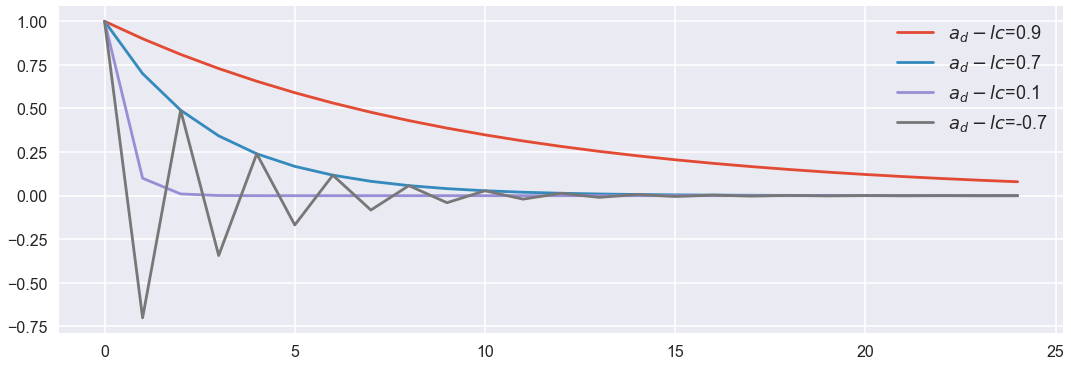
\includegraphics[width=0.8\textwidth]{fig/exponential_decay}
		\caption*{Exponential decay for different values of $a_d-lc$.}
	\end{figure}
	
	
	%\insertimptext{Convergency is guranteed for all values of $\tilde{\bm{x}}(0)$}
	
\end{frame}

\begin{frame}
    \frametitle{Example}
    True and estimated position of the car, along with the true and estimated speed.
    \movie{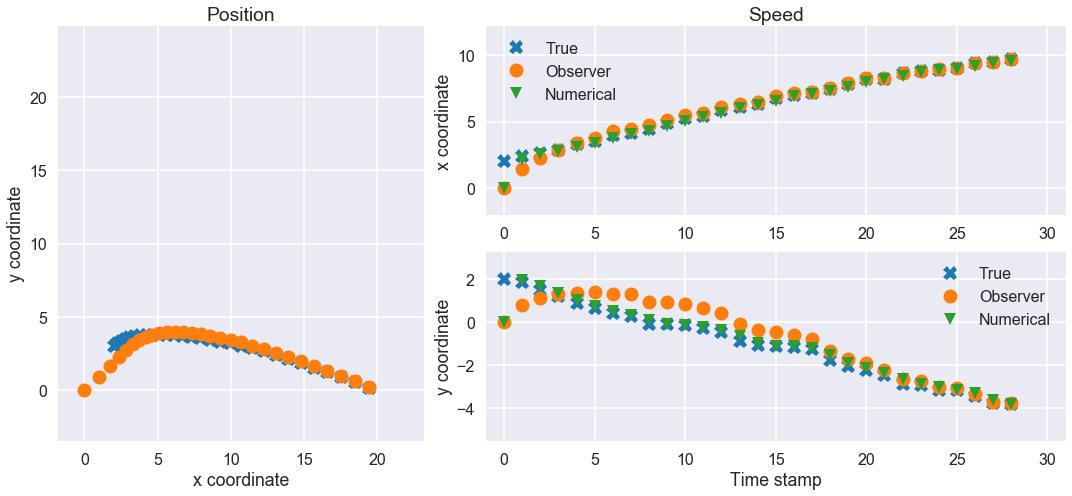
\includegraphics[width=0.8\textwidth]{fig/observer_ex_1}}{video/observer_ex_1.avi}
\end{frame}

\begin{frame}
\begin{figure}[b]
	\frametitle{Speed estimation error}
	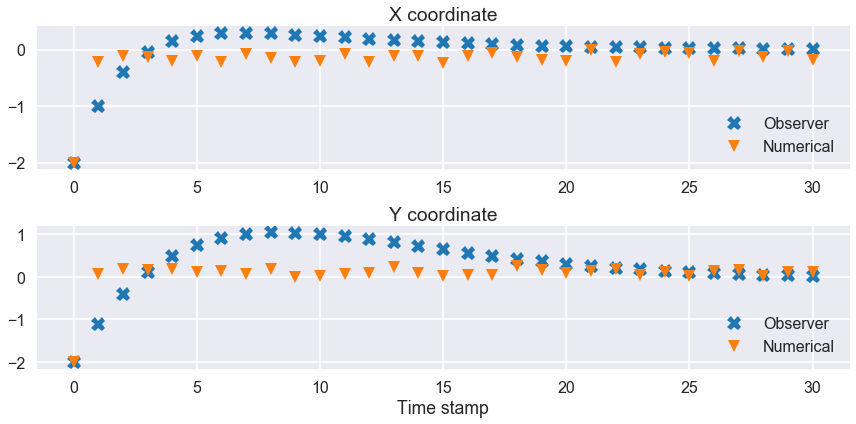
\includegraphics[width=0.8\textwidth]{fig/speed_estimation_error_ex_1}
\end{figure}
\end{frame}	

\end{document}
	